% Options for packages loaded elsewhere
\PassOptionsToPackage{unicode,linktoc=all,pdfwindowui,pdfpagemode=FullScreen}{hyperref}
\PassOptionsToPackage{hyphens}{url}
\PassOptionsToPackage{dvipsnames,svgnames,x11names}{xcolor}
%
\documentclass[
  letterpaper,
  twoside,
  openright,
  headsepline,
  footsepline,
  listof = totocnumbered,
  chapterprefix = true,
  titlepage = false]{scrbook}

\usepackage{amsmath,amssymb}
\usepackage{iftex}
\ifPDFTeX
  \usepackage[T1]{fontenc}
  \usepackage[utf8]{inputenc}
  \usepackage{textcomp} % provide euro and other symbols
\else % if luatex or xetex
  \usepackage{unicode-math}
  \defaultfontfeatures{Scale=MatchLowercase}
  \defaultfontfeatures[\rmfamily]{Ligatures=TeX,Scale=1}
\fi
\usepackage{lmodern}
\ifPDFTeX\else  
    % xetex/luatex font selection
\fi
% Use upquote if available, for straight quotes in verbatim environments
\IfFileExists{upquote.sty}{\usepackage{upquote}}{}
\IfFileExists{microtype.sty}{% use microtype if available
  \usepackage[]{microtype}
  \UseMicrotypeSet[protrusion]{basicmath} % disable protrusion for tt fonts
}{}
\makeatletter
\@ifundefined{KOMAClassName}{% if non-KOMA class
  \IfFileExists{parskip.sty}{%
    \usepackage{parskip}
  }{% else
    \setlength{\parindent}{0pt}
    \setlength{\parskip}{6pt plus 2pt minus 1pt}}
}{% if KOMA class
  \KOMAoptions{parskip=half}}
\makeatother
\usepackage{xcolor}
\usepackage[lmargin=1in,rmargin=1in,tmargin=1in,bmargin=1in]{geometry}
\setlength{\emergencystretch}{3em} % prevent overfull lines
\setcounter{secnumdepth}{3}
% Make \paragraph and \subparagraph free-standing
\ifx\paragraph\undefined\else
  \let\oldparagraph\paragraph
  \renewcommand{\paragraph}[1]{\oldparagraph{#1}\mbox{}}
\fi
\ifx\subparagraph\undefined\else
  \let\oldsubparagraph\subparagraph
  \renewcommand{\subparagraph}[1]{\oldsubparagraph{#1}\mbox{}}
\fi

\usepackage{color}
\usepackage{fancyvrb}
\newcommand{\VerbBar}{|}
\newcommand{\VERB}{\Verb[commandchars=\\\{\}]}
\DefineVerbatimEnvironment{Highlighting}{Verbatim}{commandchars=\\\{\}}
% Add ',fontsize=\small' for more characters per line
\usepackage{framed}
\definecolor{shadecolor}{RGB}{241,243,245}
\newenvironment{Shaded}{\begin{snugshade}}{\end{snugshade}}
\newcommand{\AlertTok}[1]{\textcolor[rgb]{0.68,0.00,0.00}{#1}}
\newcommand{\AnnotationTok}[1]{\textcolor[rgb]{0.37,0.37,0.37}{#1}}
\newcommand{\AttributeTok}[1]{\textcolor[rgb]{0.40,0.45,0.13}{#1}}
\newcommand{\BaseNTok}[1]{\textcolor[rgb]{0.68,0.00,0.00}{#1}}
\newcommand{\BuiltInTok}[1]{\textcolor[rgb]{0.00,0.23,0.31}{#1}}
\newcommand{\CharTok}[1]{\textcolor[rgb]{0.13,0.47,0.30}{#1}}
\newcommand{\CommentTok}[1]{\textcolor[rgb]{0.37,0.37,0.37}{#1}}
\newcommand{\CommentVarTok}[1]{\textcolor[rgb]{0.37,0.37,0.37}{\textit{#1}}}
\newcommand{\ConstantTok}[1]{\textcolor[rgb]{0.56,0.35,0.01}{#1}}
\newcommand{\ControlFlowTok}[1]{\textcolor[rgb]{0.00,0.23,0.31}{#1}}
\newcommand{\DataTypeTok}[1]{\textcolor[rgb]{0.68,0.00,0.00}{#1}}
\newcommand{\DecValTok}[1]{\textcolor[rgb]{0.68,0.00,0.00}{#1}}
\newcommand{\DocumentationTok}[1]{\textcolor[rgb]{0.37,0.37,0.37}{\textit{#1}}}
\newcommand{\ErrorTok}[1]{\textcolor[rgb]{0.68,0.00,0.00}{#1}}
\newcommand{\ExtensionTok}[1]{\textcolor[rgb]{0.00,0.23,0.31}{#1}}
\newcommand{\FloatTok}[1]{\textcolor[rgb]{0.68,0.00,0.00}{#1}}
\newcommand{\FunctionTok}[1]{\textcolor[rgb]{0.28,0.35,0.67}{#1}}
\newcommand{\ImportTok}[1]{\textcolor[rgb]{0.00,0.46,0.62}{#1}}
\newcommand{\InformationTok}[1]{\textcolor[rgb]{0.37,0.37,0.37}{#1}}
\newcommand{\KeywordTok}[1]{\textcolor[rgb]{0.00,0.23,0.31}{#1}}
\newcommand{\NormalTok}[1]{\textcolor[rgb]{0.00,0.23,0.31}{#1}}
\newcommand{\OperatorTok}[1]{\textcolor[rgb]{0.37,0.37,0.37}{#1}}
\newcommand{\OtherTok}[1]{\textcolor[rgb]{0.00,0.23,0.31}{#1}}
\newcommand{\PreprocessorTok}[1]{\textcolor[rgb]{0.68,0.00,0.00}{#1}}
\newcommand{\RegionMarkerTok}[1]{\textcolor[rgb]{0.00,0.23,0.31}{#1}}
\newcommand{\SpecialCharTok}[1]{\textcolor[rgb]{0.37,0.37,0.37}{#1}}
\newcommand{\SpecialStringTok}[1]{\textcolor[rgb]{0.13,0.47,0.30}{#1}}
\newcommand{\StringTok}[1]{\textcolor[rgb]{0.13,0.47,0.30}{#1}}
\newcommand{\VariableTok}[1]{\textcolor[rgb]{0.07,0.07,0.07}{#1}}
\newcommand{\VerbatimStringTok}[1]{\textcolor[rgb]{0.13,0.47,0.30}{#1}}
\newcommand{\WarningTok}[1]{\textcolor[rgb]{0.37,0.37,0.37}{\textit{#1}}}

\providecommand{\tightlist}{%
  \setlength{\itemsep}{0pt}\setlength{\parskip}{0pt}}\usepackage{longtable,booktabs,array}
\usepackage{calc} % for calculating minipage widths
% Correct order of tables after \paragraph or \subparagraph
\usepackage{etoolbox}
\makeatletter
\patchcmd\longtable{\par}{\if@noskipsec\mbox{}\fi\par}{}{}
\makeatother
% Allow footnotes in longtable head/foot
\IfFileExists{footnotehyper.sty}{\usepackage{footnotehyper}}{\usepackage{footnote}}
\makesavenoteenv{longtable}
\usepackage{graphicx}
\makeatletter
\def\maxwidth{\ifdim\Gin@nat@width>\linewidth\linewidth\else\Gin@nat@width\fi}
\def\maxheight{\ifdim\Gin@nat@height>\textheight\textheight\else\Gin@nat@height\fi}
\makeatother
% Scale images if necessary, so that they will not overflow the page
% margins by default, and it is still possible to overwrite the defaults
% using explicit options in \includegraphics[width, height, ...]{}
\setkeys{Gin}{width=\maxwidth,height=\maxheight,keepaspectratio}
% Set default figure placement to htbp
\makeatletter
\def\fps@figure{htbp}
\makeatother

\usepackage[automark]{scrlayer-scrpage}
%\usepackage[blocks]{authblk)
%\usepackage{uni-titlepage}

\providecommand{\abstractname}{Learning Objectives} % not in scrbook class
\newenvironment{objectives}[1]{%
	\hrule
	\vspace{5pt}
	\small\textbf{\abstractname: } 
	\newline
	\vspace{0.1cm}
	%\small\emph #1     %  emph takes an argument
	\small\emph{#1} % or \small\textit{#1} 
	\itshape % use this if you want the text to be in italics
}{%
	\vspace{5pt}
	\hrule
	\vspace{0.6cm}
}
\AtBeginDocument{%
\begin{titlepage}
	\centering
	\vspace*{\baselineskip}
	\rule{\textwidth}{1.6pt}\vspace*{-\baselineskip}\vspace*{2pt}
	\rule{\textwidth}{0.4pt}\\[\baselineskip]
	{\LARGE Regression Analysis\\ With \\[0.3\baselineskip] R And Easystats}\\[0.2\baselineskip]
	\rule{\textwidth}{0.4pt}\vspace*{-\baselineskip}\vspace{3.2pt}
	\rule{\textwidth}{1.6pt}\\[\baselineskip]
	\scshape
	\vspace*{8\baselineskip}
	Author \\[\baselineskip]
	{\Large Maulik Bhatt \par}
	{\itshape S P Jain Institute of Management \& Research \\ Mumbai\par}
	\vfill
	{\scshape 2023} \\
	{\large Maulik Bhatt}\par%
\end{titlepage}
}
\makeatletter
\makeatother
\makeatletter
\@ifpackageloaded{bookmark}{}{\usepackage{bookmark}}
\makeatother
\makeatletter
\@ifpackageloaded{caption}{}{\usepackage{caption}}
\AtBeginDocument{%
\ifdefined\contentsname
  \renewcommand*\contentsname{Table of contents}
\else
  \newcommand\contentsname{Table of contents}
\fi
\ifdefined\listfigurename
  \renewcommand*\listfigurename{List of Figures}
\else
  \newcommand\listfigurename{List of Figures}
\fi
\ifdefined\listtablename
  \renewcommand*\listtablename{List of Tables}
\else
  \newcommand\listtablename{List of Tables}
\fi
\ifdefined\figurename
  \renewcommand*\figurename{Figure}
\else
  \newcommand\figurename{Figure}
\fi
\ifdefined\tablename
  \renewcommand*\tablename{Table}
\else
  \newcommand\tablename{Table}
\fi
}
\@ifpackageloaded{float}{}{\usepackage{float}}
\floatstyle{ruled}
\@ifundefined{c@chapter}{\newfloat{codelisting}{h}{lop}}{\newfloat{codelisting}{h}{lop}[chapter]}
\floatname{codelisting}{Listing}
\newcommand*\listoflistings{\listof{codelisting}{List of Listings}}
\makeatother
\makeatletter
\@ifpackageloaded{caption}{}{\usepackage{caption}}
\@ifpackageloaded{subcaption}{}{\usepackage{subcaption}}
\makeatother
\makeatletter
\@ifpackageloaded{tcolorbox}{}{\usepackage[skins,breakable]{tcolorbox}}
\makeatother
\makeatletter
\@ifundefined{shadecolor}{\definecolor{shadecolor}{rgb}{.97, .97, .97}}
\makeatother
\makeatletter
\makeatother
\makeatletter
\makeatother
\ifLuaTeX
  \usepackage{selnolig}  % disable illegal ligatures
\fi
\IfFileExists{bookmark.sty}{\usepackage{bookmark}}{\usepackage{hyperref}}
\IfFileExists{xurl.sty}{\usepackage{xurl}}{} % add URL line breaks if available
\urlstyle{same} % disable monospaced font for URLs
\hypersetup{
  pdftitle={Regression Analysis With R and Easystats},
  pdfauthor={Maulik Bhatt},
  colorlinks=true,
  linkcolor={Maroon},
  filecolor={Maroon},
  citecolor={Blue},
  urlcolor={Blue},
  pdfcreator={LaTeX via pandoc}}

\title{Regression Analysis With R and Easystats}
\author{Maulik Bhatt}
\date{26/06/2023}

\begin{document}
\frontmatter
\maketitle
\ifdefined\Shaded\renewenvironment{Shaded}{\begin{tcolorbox}[interior hidden, borderline west={3pt}{0pt}{shadecolor}, enhanced, breakable, boxrule=0pt, frame hidden, sharp corners]}{\end{tcolorbox}}\fi

\renewcommand*\contentsname{Contents}
{
\hypersetup{linkcolor=}
\setcounter{tocdepth}{2}
\tableofcontents
}
\listoffigures
\listoftables
\mainmatter
\bookmarksetup{startatroot}

\hypertarget{preface}{%
\chapter*{Preface}\label{preface}}
\addcontentsline{toc}{chapter}{Preface}

\markboth{Preface}{Preface}

\bookmarksetup{startatroot}

\hypertarget{acknowledgement}{%
\chapter*{Acknowledgement}\label{acknowledgement}}
\addcontentsline{toc}{chapter}{Acknowledgement}

\markboth{Acknowledgement}{Acknowledgement}

I would like to express my heartfelt gratitude to the individuals who
have played a significant role in the creation of this book on
Regression Analysis with R. Their guidance, knowledge, and support have
been invaluable throughout this journey.

First and foremost, I extend my deepest appreciation to my esteemed
professors, {[}Professor's Name{]}, {[}Professor's Name{]}, and
{[}Professor's Name{]}. Their expertise in statistics and econometrics
has shaped my understanding of quantitative analysis and provided a
solid foundation for this book. Their dedication to teaching and their
unwavering commitment to fostering academic excellence have been
instrumental in my growth as a student of econometrics.

I would like to extend special thanks to my colleague and dear friend,
{[}Colleague's Name{]}. Their introduction to the world of R programming
language opened up a world of possibilities for me. Their patience,
willingness to share their knowledge, and countless hours spent
assisting me with R-related challenges have been indispensable. I am
grateful for their unwavering support and the collaborative environment
we fostered, which significantly enriched my learning experience.

A heartfelt appreciation goes to the developers of R, an open-source
programming language that has revolutionized the field of data analysis
and statistical computing. Their tireless efforts in creating and
continuously improving R have made it an indispensable tool for
researchers and analysts worldwide. Without their dedication, this book
would not have been possible.

I would also like to express my gratitude to the developers of the R
packages that have been instrumental in the analysis and visualization
techniques presented in this book. Their commitment to excellence,
innovation, and user-friendly implementations has immensely contributed
to the field of regression analysis. Their packages have not only
expanded the capabilities of R but have also facilitated the seamless
integration of econometric methodologies into practical applications.

Finally, I extend my heartfelt thanks to my family and friends who have
supported me throughout this writing process. Their encouragement,
understanding, and belief in my abilities have been a constant source of
motivation.

To all those mentioned above, and to anyone else who has contributed to
this book in any way, I offer my deepest appreciation. Your guidance,
knowledge, and support have been invaluable in shaping this work and
have helped me fulfill my goal of sharing the beauty and importance of
regression analysis with R.

Thank you.

{[}Your Name{]}

\bookmarksetup{startatroot}

\hypertarget{introduction}{%
\chapter{Introduction}\label{introduction}}

\begin{longtable}[]{@{}
  >{\centering\arraybackslash}p{(\columnwidth - 0\tabcolsep) * \real{1.0000}}@{}}
\toprule\noalign{}
\begin{minipage}[b]{\linewidth}\centering
Status
\end{minipage} \\
\midrule\noalign{}
\endhead
\bottomrule\noalign{}
\endlastfoot
This chapter is currently a dumping ground for ideas, and we don't
recommend reading it. \\
\end{longtable}

\begin{objectives}{In this chapter, you will learn to}
\begin{itemize}

\item{Importance of regression analysis in econometrics}

\item{Overview of the book's structure and goals}

\item{Introduction to R programming language and its relevance to econometric analysis}

\end{itemize}

\end{objectives}

Econometrics is a combination of two words: Econo + Metric. Econo refers
to concepts of economics, while metric refers to measurement. Let's take
an example of the law of demand from microeconomic theory. We know the
demand of a commodity will decrease if the price of the commodity
increases. But we don't know how much the demand will decrease, given
the increase in the price is one unit (i.e., one Dollar, or one Euro,
etc.). In Econometrics, we measure such increase or decrease using
various experiments. In these experiments, we observe how much the
demand for a commodity increase of decrease in response to a unit change
(increase or decrease) in price of the commodity.

\hypertarget{importance-of-r-for-econometrics-and-statistics}{%
\section{Importance of R for Econometrics and
Statistics}\label{importance-of-r-for-econometrics-and-statistics}}

Many software are available for statistical and econometric analysis.
Some of the popular software include SPSS, SAS, Stata, MATLAB, etc.
These are all proprietary software. Free and open source alternatives
include python and R, which are programming languages. The users need to
type the commands in order to perform various tasks/analysis in these
programming languages.

Python is a general purpose programming langauge, while R is a
statistical programming language. R also has many packages (i.e.,
add-ons, which enhance the functionality of R). As of writing this,
there are \texttt{19697} packages available on CRAN (the Comprehensive R
Archive Network, which is the central authority to decide about R
programming language). Even more packages are available on
\texttt{github}, which is an Internet hosting service for software
development and version control using the version control system Git.
Because of such extensive support, I have chosen R to conduct
econometric analysis for this book.

In particular, I will use \texttt{easystats} set of packages, which are
designed for various statistical analysis tasks. We will see how
\texttt{easystats} make our tasks easier in R.

I will also use \texttt{quarto}, which is a document preparation system,
based on pandoc's markdown. The benefit of \texttt{quarto} is that we
can keep our analysis and prose in the same document. At the end, when
we click on the \texttt{build} button, it renders the entire book in
either pdf or HTML format. It is also possible to render the book in
Microsoft Word format, but this output format has got limited support.
It is more convenient to design and customize the output in HTML and PDF
formats. We will discuss more about this in the chapter of Getting
Started with R.

\bookmarksetup{startatroot}

\hypertarget{introduction-to-econometrics-and-regression-analysis}{%
\chapter{Introduction to Econometrics and Regression
Analysis}\label{introduction-to-econometrics-and-regression-analysis}}

\begin{longtable}[]{@{}
  >{\centering\arraybackslash}p{(\columnwidth - 0\tabcolsep) * \real{1.0000}}@{}}
\toprule\noalign{}
\begin{minipage}[b]{\linewidth}\centering
Status
\end{minipage} \\
\midrule\noalign{}
\endhead
\bottomrule\noalign{}
\endlastfoot
This chapter is currently a dumping ground for ideas, and we don't
recommend reading it. \\
\end{longtable}

\begin{objectives}{In this chapter, you will learn to}
\begin{itemize}

\item{Understanding the basics of econometrics}

\item{Role of regression analysis in econometric modeling}

\item{Overview of the regression analysis process}

\item{Introduction to R for econometric analysis}

\end{itemize}

\end{objectives}

Basics of Econometrics

Role of Regression

Introduction to R

\bookmarksetup{startatroot}

\hypertarget{getting-started-with-r-for-econometrics}{%
\chapter{Getting Started with R for
Econometrics}\label{getting-started-with-r-for-econometrics}}

\begin{longtable}[]{@{}
  >{\centering\arraybackslash}p{(\columnwidth - 0\tabcolsep) * \real{1.0000}}@{}}
\toprule\noalign{}
\begin{minipage}[b]{\linewidth}\centering
Status
\end{minipage} \\
\midrule\noalign{}
\endhead
\bottomrule\noalign{}
\endlastfoot
This chapter is currently a dumping ground for ideas, and we don't
recommend reading it. \\
\end{longtable}

\begin{objectives}{In this chapter, you will learn to}
\begin{itemize}

\item{Introduction to R programming language and its ecosystem}

\item{Setting up the R environment and installing necessary packages}

\item{Loading and manipulating data in R for econometric analysis}

\item{Exploring data visualization techniques using R}

\end{itemize}

\end{objectives}

\hypertarget{a-brief-history-of-r}{%
\section{A Brief History of R}\label{a-brief-history-of-r}}

John Chambers, working at Bell Laboratories, developed S programming
language for statistical analysis. This programming language was
incorporated in the commercial program S-plus. Inspired by this
programming languagage, tw o statistics professors Robert Gentleman and
Ross Ihaka developed a reduced version of S, which they named R.

R was first released in 1993. In 1995, another statistician Martin
Mächler convinced Gentleman and Ihaka to make R source code available to
general public. As a result, R became free and open source under GNU
General Public License.

R also has a robust community of users. As of writing this, there are
19,719 user-developed packages on Comprehensive R Archive Network
(CRAN), which distributes the R source code and packages. Apart from
CRAN, many more packages are also available on code sharing platform
github. Users can download packages from github as well. The Appendix A
explains how to install packages from CRAN and from github.

How to Install R

You can install R from the website of
\href{https://cran.r-project.org/}{CRAN}. Downloadable files and
instructions to download and install R for all the major operating
systems are available on this website. R can be downloaded and installed
on Windows, Mac and Linux platforms.

It is possible to use R right from within this R Graphical User
Interface (R-Gui). But such a work will not be reproducible. It means,
you will be able to work on your system, but you won't be able to share
that work with others. IDE like RStudio makes it much easier to work in
R, and to share your work with others.

How to Install RStudio

Once you have installed R for your operating system, you can visit the
website of \href{https://posit.co/download/rstudio-desktop/}{RStudio}.
Just like R, RStudio is also available on Windows, Mac and Linux
platforms.

Useful Settings in RStudio

I would recommend you not to save the workspace in RStudio. This setting
can be disabled in RStudio as follows:

\begin{figure}

{\centering 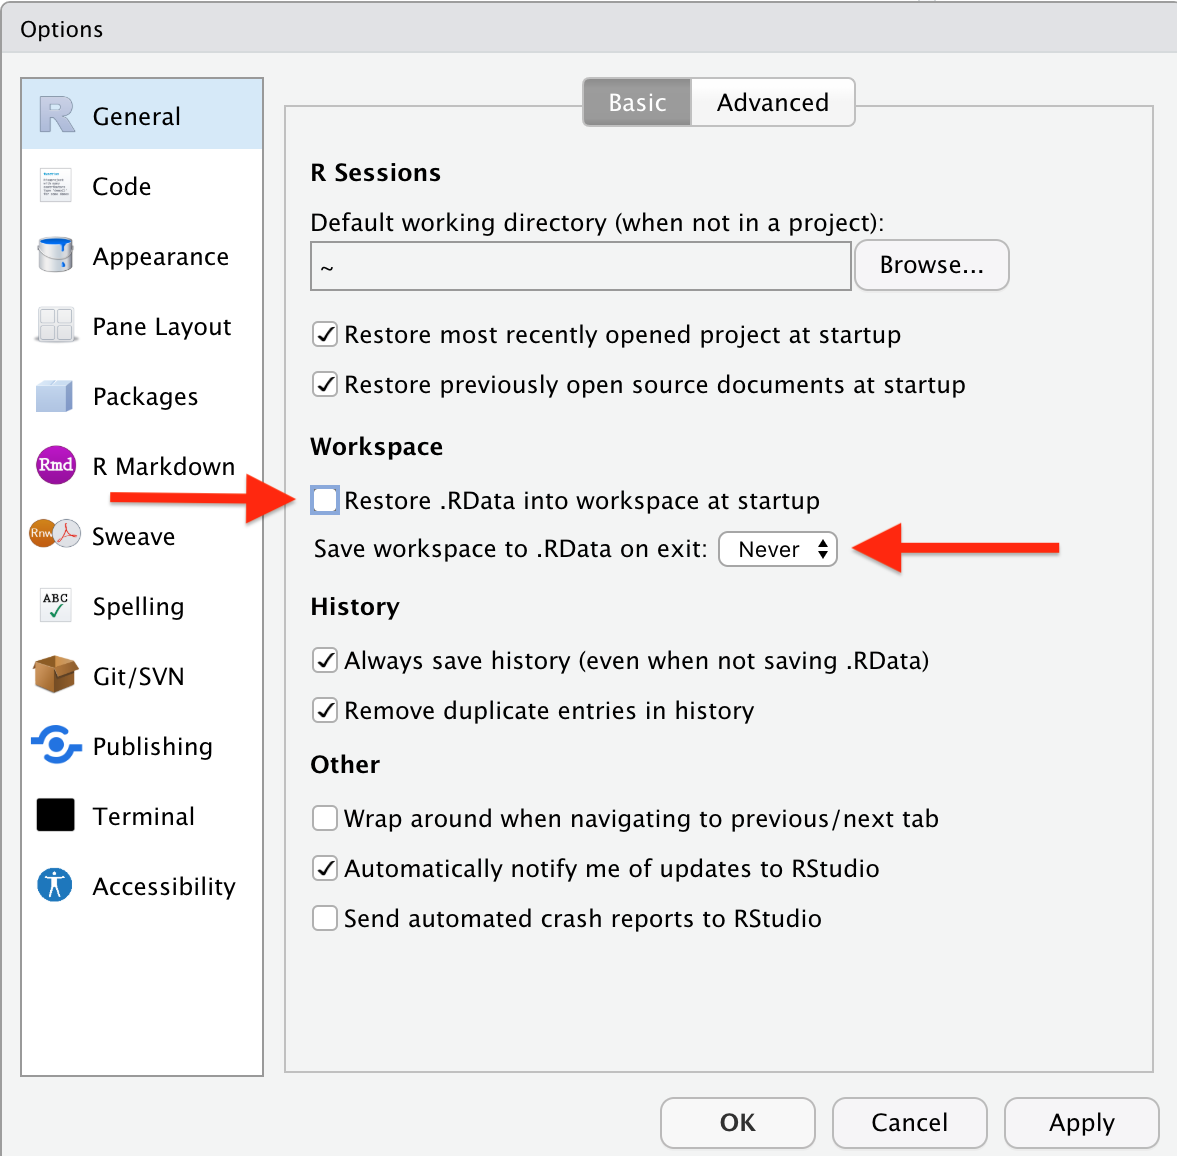
\includegraphics[width=3.92in,height=\textheight]{images/RStudio-settings.png}

}

\caption{\label{fig-disable-workspace}How to Disable Saving Workspace}

\end{figure}

This setting (of not saving your workspace) seems counter-intuitive. But
it helps you in the longer term. Assume you have to share your work with
someone else. The other person might not have the same settings of
computer in his/her system. So, the work on your system might look
different in that system. Instead, you should save the R Script (or even
better, a Quarto document) in your system, and should share it.

The Concept of Working Directory

R has a concept of working directory. When you save your R script and
your work, it gets saved in the ``working directory'' of R. You can find
and change the working directory using R commands.

\begin{Shaded}
\begin{Highlighting}[numbers=left,,]
\CommentTok{\# Find the working directory}
\FunctionTok{getwd}\NormalTok{()}
\CommentTok{\#Change the working directory}
\FunctionTok{setwd}\NormalTok{(}\StringTok{"Path/to/another/folder"}\NormalTok{)}
\end{Highlighting}
\end{Shaded}

Quarto

Quarto is a new open-source scientific and technical publishing system
developed by Posit (the maker of RStudio). Quarto is designed to be
useful to anyone who wants to create reproducible documents. A Quarto
document contains both - the code and the prose. For example, if you are
running regression analysis in R, R Script will only contain your code,
but a Quarto document will contain your R code and your interpretation
of the regression results. Quarto runs computations into separate
pluggable language ``engines'', which helps make this cross-language
functionality easier to support .

Here are some points that emphasize the reproducibility of Quarto over R
scripts:

\begin{enumerate}
\def\labelenumi{\arabic{enumi}.}
\item
  \textbf{Cross-language support}: Quarto is designed to work with
  multiple languages, including Python, bash, Julia, C, SQL, and more.
  This makes it easier to work with different languages in the same
  document.
\item
  \textbf{Built-in output formats}: Quarto generates the output in
  various formats like Microsoft Word, HTML, PDF, beamer, revealjs, etc.
  It also has many options for customizing each format.
\item
  \textbf{Native features for special project types}: Quarto has native
  features for special project types like websites, books, and blogs.
  This means that you don't have to rely on external packages. As a
  matter of fact, this book is written entirely using Quarto in RStudio.
\item
  \textbf{Easier rendering}: Quarto isn't an R package. It's a
  command-line interface that makes it much easier to work with Quarto
  documents outside of the RStudio IDE. You can also use Quarto in other
  IDEs like VS Code.
\end{enumerate}

These features make Quarto a better choice than R scripts when it comes
to reproducibility. With Quarto, you can easily create documents that
are easy to reproduce and share with others.

Optional: Installing \LaTeX

If you want to work in Quarto, and want to generate PDF output,
\LaTeX is required. There are two popular \LaTeX distributions: MiKTeX
and TeX Live. However, I prefer another \LaTeX distribution, called
TinyTeX. It's a light weight distribution of \LaTeX, and works well with
R. You can install it using R as follows:

\begin{Shaded}
\begin{Highlighting}[numbers=left,,]
\CommentTok{\#install tinytex R package}
\FunctionTok{install.packages}\NormalTok{(}\StringTok{"tinytex"}\NormalTok{)}
\CommentTok{\#load it in R}
\FunctionTok{library}\NormalTok{(tinytex)}
\CommentTok{\#use this package to install LaTeX compiler TinyTeX}
\FunctionTok{install\_tinytex}\NormalTok{()}
\end{Highlighting}
\end{Shaded}

These commands install the most commonly used \LaTeX packages into your
system. However, if you want to install all the \LaTeX packages, you can
do so by using \texttt{install\_tinytex(bundle\ =\ "TinyTeX-2")} instead
of \texttt{install\_tinytex()} function above.

\bookmarksetup{startatroot}

\hypertarget{simple-linear-regression}{%
\chapter{Simple Linear Regression}\label{simple-linear-regression}}

\begin{longtable}[]{@{}
  >{\centering\arraybackslash}p{(\columnwidth - 0\tabcolsep) * \real{1.0000}}@{}}
\toprule\noalign{}
\begin{minipage}[b]{\linewidth}\centering
Status
\end{minipage} \\
\midrule\noalign{}
\endhead
\bottomrule\noalign{}
\endlastfoot
This chapter is currently a dumping ground for ideas, and we don't
recommend reading it. \\
\end{longtable}

\begin{objectives}{In this chapter, you will learn to}
\begin{itemize}

\item{Understanding the principles of simple linear regression}

\item{Performing simple linear regression in R for econometric analysis}

\item{Interpreting regression results in the context of economic variables}

\item{Assessing model assumptions and addressing violations}

\item{Practical examples and exercises using R}

\end{itemize}

\end{objectives}

\begin{Shaded}
\begin{Highlighting}[numbers=left,,]
\FunctionTok{library}\NormalTok{(easystats)}
\FunctionTok{library}\NormalTok{(ggplot2)}
\end{Highlighting}
\end{Shaded}

Introduction

Linear regression is among the fundamental concepts in Econometrics. In
linear regression, we try to estimate how much one variable will change,
with response to a change in another variable. The controlled variable
is called predictor or independent variable. The variable, which changes
as a response to a change in the controlled variable is called response
or dependent variable. In R, we denote such relationship with
\texttt{y\textasciitilde{}x}, where y is the response and x is the
predictor. The notation \texttt{y\textasciitilde{}x} is read as ``y
explained by x''.

In mathematical terms, we are fitting a linear equation between x and y.
When we write \texttt{y\textasciitilde{}x}, it means
\texttt{y\ =\ ax\ +\ b}, and we need to find a and b from the data
points given.

Let's understand what it means for us. The workflow for the linear
regression problem would be:

\begin{enumerate}
\def\labelenumi{\arabic{enumi}.}
\item
  We would be given some observations of both - independent variable and
  dependent variable.
\item
  we graph these data points, using a coordinate system (like Cartesian
  system). Each value is represented by a dot. Such a diagram is called
  a scatter-plot diagram.
\item
  After graphing the points onto a scatter plot diagram, linear
  regression analysis seeks to find the best-fit line to fit the points
  as closely as possible.
\item
  This best-fit line is a line, which minimizes the distance between the
  points falling above or below the lines.
\end{enumerate}

\href{https://www.fiverr.com/resources/guides/data/linear-regression-101}{Linear
Regression 101: What Is It And How Is It Done? \textbar{} Fiverr}

Principles of Linear Regression (Gauss Markov)

Example in R

For understanding regression, we can generate a dummy dataset, and
create a regression model on the basis of the data.

\begin{Shaded}
\begin{Highlighting}[numbers=left,,]
\NormalTok{dummy }\OtherTok{\textless{}{-}} \FunctionTok{data.frame}\NormalTok{(}\AttributeTok{y =} \FunctionTok{rnorm}\NormalTok{(}\DecValTok{100}\NormalTok{),}\AttributeTok{x =} \FunctionTok{rpois}\NormalTok{(}\DecValTok{100}\NormalTok{,}\DecValTok{3}\NormalTok{))}
\end{Highlighting}
\end{Shaded}

In the code above, we have created a dummy data. The \texttt{rnorm(n)}
function generates n number of data points based on normal distribution.
The default mean and standard deviation are 0 and 1 respectively.
Similarly, the \texttt{rpois(n,l)} function generates n number of data
points based on poisson distribution, with \lambda = l. We can plot the
data to explore it visually. We will use \texttt{ggplot2} package to
create this scatterplot diagram.

\begin{Shaded}
\begin{Highlighting}[numbers=left,,]
\FunctionTok{ggplot}\NormalTok{(dummy)}\SpecialCharTok{+}\FunctionTok{aes}\NormalTok{(x,y)}\SpecialCharTok{+}\FunctionTok{geom\_point}\NormalTok{()}\SpecialCharTok{+}\FunctionTok{labs}\NormalTok{(}\AttributeTok{title =} \StringTok{"Scatterplot Diagram of X and Y"}\NormalTok{)}
\end{Highlighting}
\end{Shaded}

\begin{figure}[H]

{\centering 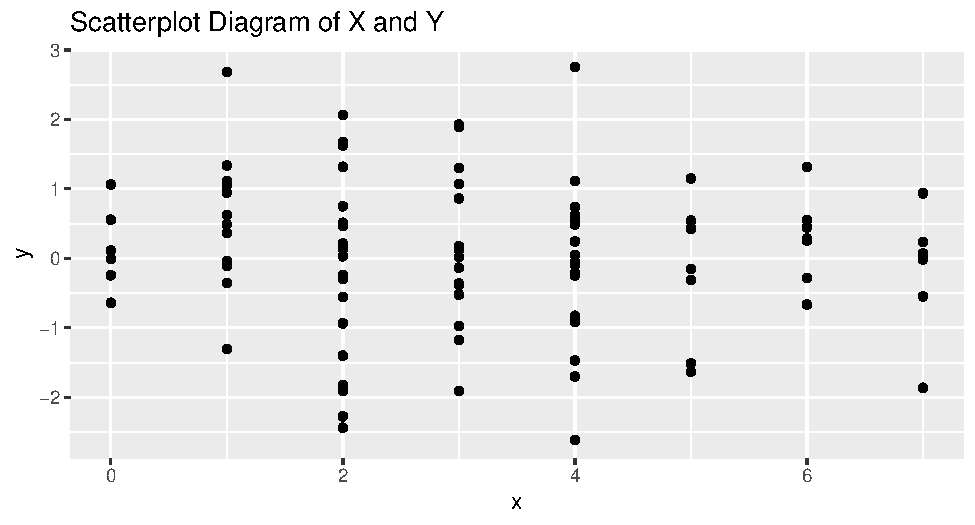
\includegraphics{lm_files/figure-pdf/fig-scatterplot-1.pdf}

}

\caption{\label{fig-scatterplot}Scatterplot of X and Y}

\end{figure}

Now we can create a regression model from this dataset.

\begin{Shaded}
\begin{Highlighting}[numbers=left,,]
\NormalTok{model1 }\OtherTok{\textless{}{-}} \FunctionTok{lm}\NormalTok{(y}\SpecialCharTok{\textasciitilde{}}\NormalTok{x, }\AttributeTok{data =}\NormalTok{ dummy)}
\end{Highlighting}
\end{Shaded}

This model stores a lot of information, but it is difficult to
understand and get the meaning out of it. So, one way is to use the
\texttt{summary} function on this \texttt{model1} object.

\begin{Shaded}
\begin{Highlighting}[numbers=left,,]
\FunctionTok{summary}\NormalTok{(model1)}
\end{Highlighting}
\end{Shaded}

\begin{verbatim}

Call:
lm(formula = y ~ x, data = dummy)

Residuals:
    Min      1Q  Median      3Q     Max 
-2.6342 -0.4445  0.0324  0.6090  2.7336 

Coefficients:
            Estimate Std. Error t value Pr(>|t|)
(Intercept)  0.24693    0.20632   1.197    0.234
x           -0.05627    0.05672  -0.992    0.324

Residual standard error: 1.051 on 98 degrees of freedom
Multiple R-squared:  0.009944,  Adjusted R-squared:  -0.0001589 
F-statistic: 0.9843 on 1 and 98 DF,  p-value: 0.3236
\end{verbatim}

The problem with this summary object is that it is not a data.frame. It
is difficult to put this object in a research paper or any other
academic submisison. So, we can use the \texttt{easystats} packages for
this. The \texttt{model\_parameters} function would show us the
parameters (aka coefficients) of the model, and the
\texttt{model\_performance} function will show us the effectiveness of
the regression model. We can also use the \texttt{display} function to
beautify the table in the output.

\begin{Shaded}
\begin{Highlighting}[numbers=left,,]
\NormalTok{model1 }\SpecialCharTok{|\textgreater{}} \FunctionTok{model\_parameters}\NormalTok{() }\SpecialCharTok{|\textgreater{}} 
  \FunctionTok{display}\NormalTok{(}\AttributeTok{format =} \StringTok{"markdown"}\NormalTok{, }\AttributeTok{caption =} \StringTok{"Regression Parameters"}\NormalTok{)}
\end{Highlighting}
\end{Shaded}

\hypertarget{tbl-regression-params}{}
\begin{longtable}[]{@{}lccccc@{}}
\caption{\label{tbl-regression-params}Regression
Parameters}\tabularnewline
\toprule\noalign{}
Parameter & Coefficient & SE & 95\% CI & t(98) & p \\
\midrule\noalign{}
\endfirsthead
\toprule\noalign{}
Parameter & Coefficient & SE & 95\% CI & t(98) & p \\
\midrule\noalign{}
\endhead
\bottomrule\noalign{}
\endlastfoot
(Intercept) & 0.25 & 0.21 & (-0.16, 0.66) & 1.20 & 0.234 \\
x & -0.06 & 0.06 & (-0.17, 0.06) & -0.99 & 0.324 \\
\end{longtable}

\begin{Shaded}
\begin{Highlighting}[numbers=left,,]
\NormalTok{model1 }\SpecialCharTok{|\textgreater{}} \FunctionTok{model\_performance}\NormalTok{() }\SpecialCharTok{|\textgreater{}} 
  \FunctionTok{display}\NormalTok{(}\AttributeTok{format =} \StringTok{"markdown"}\NormalTok{, }\AttributeTok{caption =} \StringTok{"Regression Effectiveness"}\NormalTok{)}
\end{Highlighting}
\end{Shaded}

\hypertarget{tbl-regression-effectiveness}{}
\begin{longtable}[]{@{}lcccccc@{}}
\caption{\label{tbl-regression-effectiveness}Regression
Effectiveness}\tabularnewline
\toprule\noalign{}
AIC & AICc & BIC & R2 & R2 (adj.) & RMSE & Sigma \\
\midrule\noalign{}
\endfirsthead
\toprule\noalign{}
AIC & AICc & BIC & R2 & R2 (adj.) & RMSE & Sigma \\
\midrule\noalign{}
\endhead
\bottomrule\noalign{}
\endlastfoot
297.71 & 297.96 & 305.53 & 9.94e-03 & -1.59e-04 & 1.04 & 1.05 \\
\end{longtable}

Interpretation of Regression Model

- The intercept is statistically non-significant and negative (beta =
-0.16, 95\% CI {[}-0.59, 0.27{]}, t(98) = -0.74, p = 0.461; Std. beta =
-5.50e-18, 95\% CI {[}-0.20, 0.20{]}).

\begin{itemize}
\tightlist
\item
  The effect of x is statistically non-significant and positive (beta =
  0.07, 95\% CI {[}-0.04, 0.17{]}, t(98) = 1.24, p = 0.219; Std. beta =
  0.12, 95\% CI {[}-0.07, 0.32{]}).
\end{itemize}

The model explains a statistically not significant and very

weak proportion of variance (R\^{}2 = 0.02, F(1, 98) = 1.53, p =

0.219, adj. R\^{}2 = 5.32e-03).

\bookmarksetup{startatroot}

\hypertarget{multiple-linear-regression}{%
\chapter{Multiple Linear Regression}\label{multiple-linear-regression}}

\begin{longtable}[]{@{}
  >{\centering\arraybackslash}p{(\columnwidth - 0\tabcolsep) * \real{1.0000}}@{}}
\toprule\noalign{}
\begin{minipage}[b]{\linewidth}\centering
Status
\end{minipage} \\
\midrule\noalign{}
\endhead
\bottomrule\noalign{}
\endlastfoot
This chapter is currently a dumping ground for ideas, and we don't
recommend reading it. \\
\end{longtable}

\begin{objectives}{In this chapter, you will learn to}
\begin{itemize}

\item{Extending regression analysis to multiple independent variables}

\item{Building and interpreting multiple linear regression models in R}

\item{Handling multicollinearity and selecting significant predictors in an economic context}

\item{Model evaluation and diagnostics in econometric regression}

\item{Application of multiple linear regression in economic analysis using R}

\end{itemize}

\end{objectives}

\begin{itemize}
\item
  Extending regression analysis to multiple independent variables
\item
  Building and interpreting multiple linear regression models in R
\item
  Handling multicollinearity and selecting significant predictors in an
  economic context
\item
  Model evaluation and diagnostics in econometric regression
\item
  Application of multiple linear regression in economic analysis using R
\end{itemize}

\bookmarksetup{startatroot}

\hypertarget{regression-analysis-with-dummy-variables}{%
\chapter{Regression Analysis with Dummy
Variables}\label{regression-analysis-with-dummy-variables}}

\begin{longtable}[]{@{}
  >{\centering\arraybackslash}p{(\columnwidth - 0\tabcolsep) * \real{1.0000}}@{}}
\toprule\noalign{}
\begin{minipage}[b]{\linewidth}\centering
Status
\end{minipage} \\
\midrule\noalign{}
\endhead
\bottomrule\noalign{}
\endlastfoot
This chapter is currently a dumping ground for ideas, and we don't
recommend reading it. \\
\end{longtable}

\begin{objectives}{In this chapter, you will learn to}
\begin{itemize}

\item{Incorporating categorical variables in regression analysis}

\item{Creating and interpreting dummy variables in R}

\item{Dummy variable pitfalls and remedies in econometric modeling}

\item{Examples and case studies of dummy variable regression in economics using R}

\end{itemize}

\end{objectives}

\begin{itemize}
\item
  Incorporating categorical variables in regression analysis
\item
  Creating and interpreting dummy variables in R
\item
  Dummy variable pitfalls and remedies in econometric modeling
\item
  Examples and case studies of dummy variable regression in economics
  using R
\end{itemize}

\bookmarksetup{startatroot}

\hypertarget{heteroscedasticity-and-robust-regression}{%
\chapter{Heteroscedasticity and Robust
Regression}\label{heteroscedasticity-and-robust-regression}}

\begin{longtable}[]{@{}
  >{\centering\arraybackslash}p{(\columnwidth - 0\tabcolsep) * \real{1.0000}}@{}}
\toprule\noalign{}
\begin{minipage}[b]{\linewidth}\centering
Status
\end{minipage} \\
\midrule\noalign{}
\endhead
\bottomrule\noalign{}
\endlastfoot
This chapter is currently a dumping ground for ideas, and we don't
recommend reading it. \\
\end{longtable}

\begin{objectives}{In this chapter, you will learn to}
\begin{itemize}

\item{Understanding heteroscedasticity and its implications}

\item{Addressing heteroscedasticity using robust regression techniques in R}

\item{Interpreting robust regression results in an economic context}

\item{Practical examples and exercises showcasing robust regression in econometrics}

\end{itemize}

\end{objectives}

\begin{itemize}
\item
  Understanding heteroscedasticity and its implications
\item
  Addressing heteroscedasticity using robust regression techniques in R
\item
  Interpreting robust regression results in an economic context
\item
  Practical examples and exercises showcasing robust regression in
  econometrics
\end{itemize}

\bookmarksetup{startatroot}

\hypertarget{time-series-regression}{%
\chapter{Time Series Regression}\label{time-series-regression}}

\begin{longtable}[]{@{}
  >{\centering\arraybackslash}p{(\columnwidth - 0\tabcolsep) * \real{1.0000}}@{}}
\toprule\noalign{}
\begin{minipage}[b]{\linewidth}\centering
Status
\end{minipage} \\
\midrule\noalign{}
\endhead
\bottomrule\noalign{}
\endlastfoot
This chapter is currently a dumping ground for ideas, and we don't
recommend reading it. \\
\end{longtable}

\begin{objectives}{In this chapter, you will learn to}
\begin{itemize}

\item{Introduction to time series data in econometrics}

\item{Time series regression models in R for economic analysis}

\item{Dealing with autocorrelation and lagged variables}

\item{Forecasting with time series regression models in R}

\item{Applications of time series regression in economic forecasting}

\end{itemize}

\end{objectives}

\begin{itemize}
\item
  Introduction to time series data in econometrics
\item
  Time series regression models in R for economic analysis
\item
  Dealing with autocorrelation and lagged variables
\item
  Forecasting with time series regression models in R
\item
  Applications of time series regression in economic forecasting
\end{itemize}

\bookmarksetup{startatroot}

\hypertarget{introduction-to-logistic-regression}{%
\chapter{Introduction to Logistic
Regression}\label{introduction-to-logistic-regression}}

\begin{longtable}[]{@{}
  >{\centering\arraybackslash}p{(\columnwidth - 0\tabcolsep) * \real{1.0000}}@{}}
\toprule\noalign{}
\begin{minipage}[b]{\linewidth}\centering
Status
\end{minipage} \\
\midrule\noalign{}
\endhead
\bottomrule\noalign{}
\endlastfoot
This chapter is currently a dumping ground for ideas, and we don't
recommend reading it. \\
\end{longtable}

\begin{objectives}{In this chapter, you will learn to}
\begin{itemize}

\item{Basics of logistic regression in econometrics}

\item{Estimating logistic regression models in R}

\item{Interpreting logistic regression coefficients and odds ratios}

\item{Applications of logistic regression in economic research using R}

\end{itemize}

\end{objectives}

\begin{itemize}
\item
  Basics of logistic regression in econometrics
\item
  Estimating logistic regression models in R
\item
  Interpreting logistic regression coefficients and odds ratios
\item
  Applications of logistic regression in economic research using R
\end{itemize}

\bookmarksetup{startatroot}

\hypertarget{model-evaluation-and-selection}{%
\chapter{Model Evaluation and
Selection}\label{model-evaluation-and-selection}}

\begin{longtable}[]{@{}
  >{\centering\arraybackslash}p{(\columnwidth - 0\tabcolsep) * \real{1.0000}}@{}}
\toprule\noalign{}
\begin{minipage}[b]{\linewidth}\centering
Status
\end{minipage} \\
\midrule\noalign{}
\endhead
\bottomrule\noalign{}
\endlastfoot
This chapter is currently a dumping ground for ideas, and we don't
recommend reading it. \\
\end{longtable}

\begin{objectives}{In this chapter, you will learn to}
\begin{itemize}

\item{Evaluating model performance and goodness-of-fit measures in econometrics}

\item{Validation techniques for econometric regression models}

\item{Comparing and selecting models using information criteria}

\item{Cross-validation and bootstrapping for robust model assessment in econometrics}

\end{itemize}

\end{objectives}

\begin{itemize}
\item
  Evaluating model performance and goodness-of-fit measures in
  econometrics
\item
  Validation techniques for econometric regression models
\item
  Comparing and selecting models using information criteria
\item
  Cross-validation and bootstrapping for robust model assessment in
  econometrics
\end{itemize}

\bookmarksetup{startatroot}

\hypertarget{practical-tips-and-resources-for-econometric-regression}{%
\chapter{Practical Tips and Resources for Econometric
Regression}\label{practical-tips-and-resources-for-econometric-regression}}

\begin{longtable}[]{@{}
  >{\centering\arraybackslash}p{(\columnwidth - 0\tabcolsep) * \real{1.0000}}@{}}
\toprule\noalign{}
\begin{minipage}[b]{\linewidth}\centering
Status
\end{minipage} \\
\midrule\noalign{}
\endhead
\bottomrule\noalign{}
\endlastfoot
This chapter is currently a dumping ground for ideas, and we don't
recommend reading it. \\
\end{longtable}

\begin{objectives}{In this chapter, you will learn to}
\begin{itemize}

\item{Data preparation and preprocessing tips for econometric analysis}

\item{Handling missing data and outliers in regression analysis}

\item{Dealing with endogeneity and instrumental variables}

\item{Additional resources for further learning and practice in econometrics with R}

\end{itemize}

\end{objectives}

\begin{itemize}
\item
  Data preparation and preprocessing tips for econometric analysis
\item
  Handling missing data and outliers in regression analysis
\item
  Dealing with endogeneity and instrumental variables
\item
  Additional resources for further learning and practice in econometrics
  with R
\end{itemize}

\bookmarksetup{startatroot}

\hypertarget{conclusion}{%
\chapter{Conclusion}\label{conclusion}}

\begin{longtable}[]{@{}
  >{\centering\arraybackslash}p{(\columnwidth - 0\tabcolsep) * \real{1.0000}}@{}}
\toprule\noalign{}
\begin{minipage}[b]{\linewidth}\centering
Status
\end{minipage} \\
\midrule\noalign{}
\endhead
\bottomrule\noalign{}
\endlastfoot
This chapter is currently a dumping ground for ideas, and we don't
recommend reading it. \\
\end{longtable}

\begin{objectives}{In this chapter, you will learn to}
\begin{itemize}

\item{Summary of the key concepts covered in the book}

\item{Importance of regression analysis in econometrics and economic research}

\item{Encouragement for further exploration and application of econometric regression using R}

\end{itemize}

\end{objectives}

\begin{itemize}
\item
  Summary of the key concepts covered in the book
\item
  Importance of regression analysis in econometrics and economic
  research
\item
  Encouragement for further exploration and application of econometric
  regression using R
\end{itemize}

\cleardoublepage
\phantomsection
\addcontentsline{toc}{part}{Appendices}
\appendix

\hypertarget{appendix-a-r-packages-for-econometric-regression-analysis-and-additional-resources}{%
\chapter{Appendix A: R packages for econometric regression analysis and
additional
resources}\label{appendix-a-r-packages-for-econometric-regression-analysis-and-additional-resources}}

\setcounter{figure}{0} 
\renewcommand{\thefigure}{A.\arabic{figure}}
\setcounter{table}{0} 
\renewcommand{\thetable}{A.\arabic{table}}

This book could never be completed without using many packages. The most
notable of the packages include tidyverse, easystats, AER, lmtest, fpp3,
gujarati5sie, etc. These packages can be installed using the following
commands in R.

\begin{Shaded}
\begin{Highlighting}[numbers=left,,]
\NormalTok{RA\_packages }\OtherTok{\textless{}{-}} \FunctionTok{c}\NormalTok{(}\StringTok{"AER"}\NormalTok{,}\StringTok{"easystats"}\NormalTok{,}\StringTok{"fpp3"}\NormalTok{,}\StringTok{"lmtest"}\NormalTok{,}\StringTok{"ggthemes"}\NormalTok{,}\StringTok{"gt"}\NormalTok{,}\StringTok{"gtsummary"}\NormalTok{,}\StringTok{"patchwork"}\NormalTok{,}\StringTok{"here"}\NormalTok{,}\StringTok{"fs"}\NormalTok{, }\StringTok{"knitr"}\NormalTok{,}\StringTok{"kableExtra"}\NormalTok{)}
\FunctionTok{install.packages}\NormalTok{(RA\_packages)}
\end{Highlighting}
\end{Shaded}

The commands above install the packages into your R system. However, the
functionality of these packages are not added into your R session just
because you installed these packages. You have to load the required
packages specifically whenever you need them.

Imagine you are building a home. You have completed electrification in
your home. But just because you have a fan or an AC in your home doesn't
mean they start automatically. You have to switch on the appliance
whenever you need it. Similarly, you will have to load the R packages
into your session whenever you need those packages. You can load the
package using the \texttt{library(package\_name)} command. For example,
the command to load \texttt{easystats} set of packages would be

\begin{Shaded}
\begin{Highlighting}[numbers=left,,]
\FunctionTok{library}\NormalTok{(easystats)}
\end{Highlighting}
\end{Shaded}

When you run the \texttt{install.packages(package\_name)} command, R
installs the package from Comprehensive R Archive Network (CRAN), which
is the highest authority to decide about R. However, there are many
packages, which are not available on CRAN. These packages can be
downloaded from code sharing platform Github.

To install packages from Github, you need to install one of the three
packages first: \texttt{remotes}, \texttt{devtools} or \texttt{pak}.
After that, you can easily install packages from Github also. Apart from
such packages, the development versions of regular packages (which are
available on CRAN) can also be downloaded from Github. For example, if
you want to install the package ``gujarati5sie'', which is a package
containing data from the book ``Basic Econometrics'' written by Damodar
Gujarati and others, then you can do it as follows:

\begin{Shaded}
\begin{Highlighting}[numbers=left,,]
\CommentTok{\#Install devtools, remotes or pak}
\FunctionTok{install.packages}\NormalTok{(}\StringTok{"remotes"}\NormalTok{)}\CommentTok{\#or install.packages("devltools")\#or install.packages("pak")}
\CommentTok{\#Load the package}
\FunctionTok{library}\NormalTok{(remotes)}\CommentTok{\#or library(devtools) or library(pak)}
\CommentTok{\#download the gujarati5sie package using one of the above packages}
\NormalTok{remotes}\SpecialCharTok{::}\FunctionTok{install\_github}\NormalTok{(}\StringTok{"bhattmaulik/Gujarati5sie"}\NormalTok{)}\CommentTok{\#or devtools::install\_github("bhattmaulik/Gujarati5sie") or pak::pak("bhattmaulik/Gujarati5sie")}
\end{Highlighting}
\end{Shaded}

\hypertarget{appendix-b-data-sets-used-in-the-books-examples}{%
\chapter*{Appendix B: Data sets used in the book's
examples}\label{appendix-b-data-sets-used-in-the-books-examples}}
\addcontentsline{toc}{chapter}{Appendix B: Data sets used in the book's
examples}

\markboth{Appendix B: Data sets used in the book's examples}{Appendix B:
Data sets used in the book's examples}

\setcounter{figure}{0}
\renewcommand{\thefigure}{B.\arabic{figure}} 
\setcounter{table}{0}
\renewcommand{\thetable}{B.\arabic{table}}

\hypertarget{appendix-c-how-to-build-this-book-locally}{%
\chapter*{Appendix C: How to Build This Book
Locally}\label{appendix-c-how-to-build-this-book-locally}}
\addcontentsline{toc}{chapter}{Appendix C: How to Build This Book
Locally}

\markboth{Appendix C: How to Build This Book Locally}{Appendix C: How to
Build This Book Locally}

\setcounter{figure}{0}
\renewcommand{\thefigure}{C.\arabic{figure}}
\setcounter{table}{0}
\renewcommand{\thetable}{C.\arabic{table}}

If you want to build this book locally on your computer, please download
the entire code from Github. The first step is to visit the website
\texttt{www.github.com/bhattmaulik/RegressionAnalysis}. Here, you will
find the option to download the entire book in a zip file, as shown
below.

\begin{Shaded}
\begin{Highlighting}[numbers=left,,]
\NormalTok{knitr}\SpecialCharTok{::}\FunctionTok{include\_graphics}\NormalTok{(here}\SpecialCharTok{::}\FunctionTok{here}\NormalTok{(}\StringTok{"images"}\NormalTok{,}\StringTok{"download{-}book.png"}\NormalTok{))}
\end{Highlighting}
\end{Shaded}

\begin{figure}[H]

{\centering 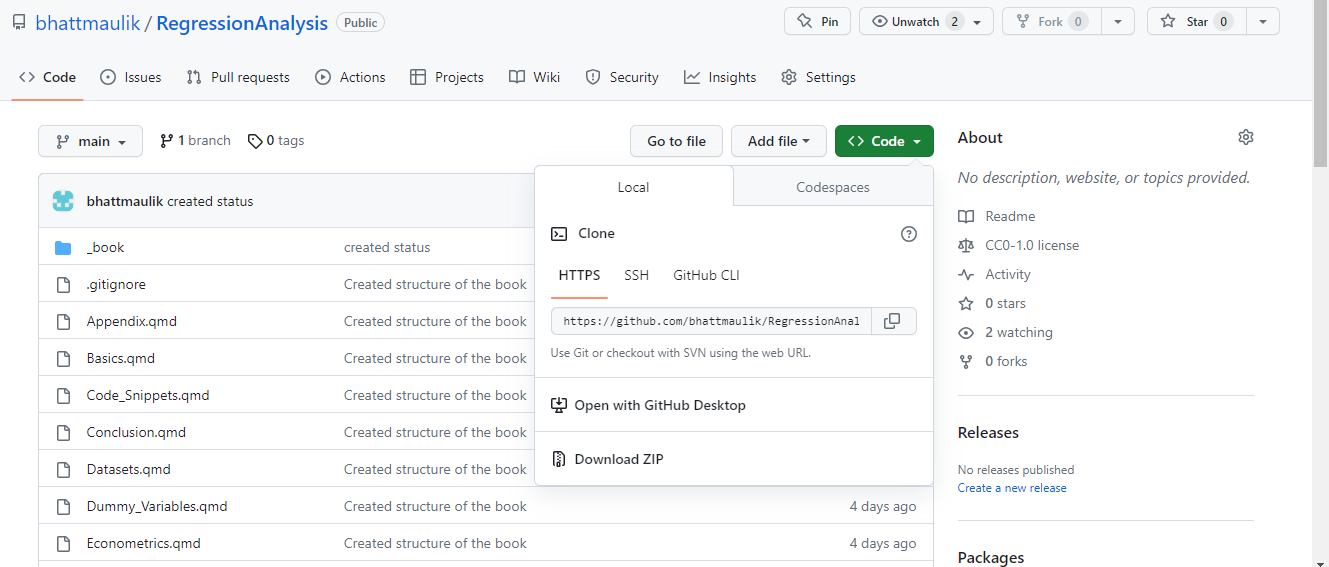
\includegraphics[width=4.43in,height=\textheight]{images/download-book.png}

}

\caption{\label{fig-download-book}Download the book from Github}

\end{figure}

After you download the zip file, unzip it. This will create a folder in
your computer. Within this folder, double click on the
``RegressionAnalysis.Rproj'' file. This will open the whole project in
RStudio.

After opening this project, go to ``Build'' pane in RStudio. This pane
is generally on the top right of RStudio along with Environment,
History, Connections, Git and Tutorial. In the build pane, click on
``\texttt{Render\ Book}'' and select ``\texttt{HTML\ format}''.

You can also choose to build the book in PDF format, but for that you
will need additional software called \texttt{tinytex}. In order to build
a book in PDF format, R also needs \texttt{LaTeX} compiler. There are
two popular \texttt{LaTeX} compilers: TeX Live and MikTeX. However, they
have their own set of problems for R users. The \texttt{LaTeX} compiler
\texttt{tinytex} attempts to solve many of them.

If you want to build the PDF book, you can install \texttt{tinytex}
through terminal in RStudio using the command
\texttt{quarto\ install\ tinytex}.

\begin{Shaded}
\begin{Highlighting}[numbers=left,,]
\NormalTok{knitr}\SpecialCharTok{::}\FunctionTok{include\_graphics}\NormalTok{(here}\SpecialCharTok{::}\FunctionTok{here}\NormalTok{(}\StringTok{"images"}\NormalTok{,}\StringTok{"build{-}book.png"}\NormalTok{))}
\end{Highlighting}
\end{Shaded}

\begin{figure}[H]

{\centering 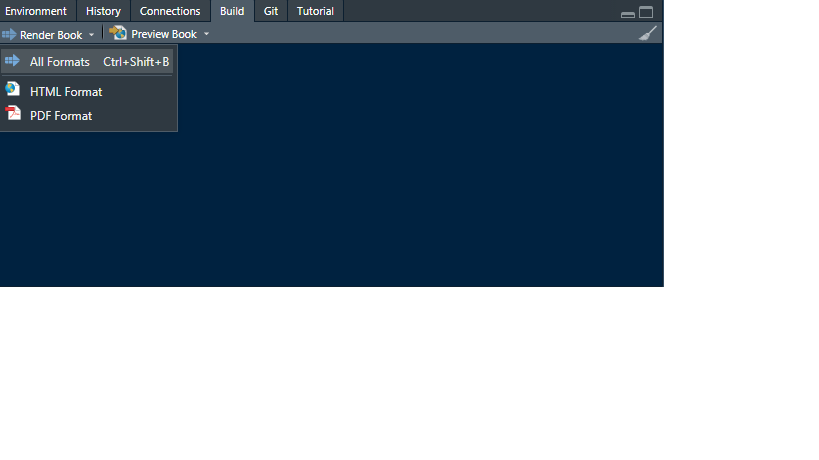
\includegraphics[width=2.73in,height=\textheight]{images/build-book.png}

}

\caption{\label{fig-build-book}Build book using tinytex}

\end{figure}

If you can't install it this way, or if you want to install it through
traditional way using R code, you can use the following code:

\begin{Shaded}
\begin{Highlighting}[numbers=left,,]
\FunctionTok{install.packages}\NormalTok{(}\StringTok{"tinytex"}\NormalTok{)}
\FunctionTok{library}\NormalTok{(tinytex)}
\NormalTok{tinytex}\SpecialCharTok{::}\FunctionTok{install\_tinytex}\NormalTok{()}
\CommentTok{\#if you want to install all the LaTeX packages, you can modify the command to tinytex::install\_tinytex(bundle = "TinyTeX{-}2")}
\end{Highlighting}
\end{Shaded}

This confuses some readers because there are two \texttt{tinytex} in
this code: the first tinytex is the \texttt{tinytex} R package. The
other \texttt{tinytex} is the \texttt{LaTeX} compiler \texttt{tinytex}.
So, when we write \texttt{library(tinytex)}, we are calling the R
package tinytex. And when we use the command \texttt{install\_tinytex},
we are installing the \texttt{LaTeX} compiler \texttt{tinytex} using the
R package \texttt{tinytex}. The benefit of this approach is that you get
to select which bundle you want to install. By default, you get to
install the bundle \texttt{TinyTeX-1}, which contains only the most
necessary LaTeX packages. But if you choose the bundle
\texttt{TinyTeX-2}, you can download all the \texttt{LaTeX} packages.


\backmatter

\end{document}
